\documentclass[twoside]{book}

% Packages required by doxygen
\usepackage{fixltx2e}
\usepackage{calc}
\usepackage{doxygen}
\usepackage[export]{adjustbox} % also loads graphicx
\usepackage{graphicx}
\usepackage[utf8]{inputenc}
\usepackage{makeidx}
\usepackage{multicol}
\usepackage{multirow}
\PassOptionsToPackage{warn}{textcomp}
\usepackage{textcomp}
\usepackage[nointegrals]{wasysym}
\usepackage[table]{xcolor}

% Font selection
\usepackage[T1]{fontenc}
\usepackage[scaled=.90]{helvet}
\usepackage{courier}
\usepackage{amssymb}
\usepackage{sectsty}
\renewcommand{\familydefault}{\sfdefault}
\allsectionsfont{%
  \fontseries{bc}\selectfont%
  \color{darkgray}%
}
\renewcommand{\DoxyLabelFont}{%
  \fontseries{bc}\selectfont%
  \color{darkgray}%
}
\newcommand{\+}{\discretionary{\mbox{\scriptsize$\hookleftarrow$}}{}{}}

% Page & text layout
\usepackage{geometry}
\geometry{%
  a4paper,%
  top=2.5cm,%
  bottom=2.5cm,%
  left=2.5cm,%
  right=2.5cm%
}
\tolerance=750
\hfuzz=15pt
\hbadness=750
\setlength{\emergencystretch}{15pt}
\setlength{\parindent}{0cm}
\setlength{\parskip}{3ex plus 2ex minus 2ex}
\makeatletter
\renewcommand{\paragraph}{%
  \@startsection{paragraph}{4}{0ex}{-1.0ex}{1.0ex}{%
    \normalfont\normalsize\bfseries\SS@parafont%
  }%
}
\renewcommand{\subparagraph}{%
  \@startsection{subparagraph}{5}{0ex}{-1.0ex}{1.0ex}{%
    \normalfont\normalsize\bfseries\SS@subparafont%
  }%
}
\makeatother

% Headers & footers
\usepackage{fancyhdr}
\pagestyle{fancyplain}
\fancyhead[LE]{\fancyplain{}{\bfseries\thepage}}
\fancyhead[CE]{\fancyplain{}{}}
\fancyhead[RE]{\fancyplain{}{\bfseries\leftmark}}
\fancyhead[LO]{\fancyplain{}{\bfseries\rightmark}}
\fancyhead[CO]{\fancyplain{}{}}
\fancyhead[RO]{\fancyplain{}{\bfseries\thepage}}
\fancyfoot[LE]{\fancyplain{}{}}
\fancyfoot[CE]{\fancyplain{}{}}
\fancyfoot[RE]{\fancyplain{}{\bfseries\scriptsize Generated by Doxygen }}
\fancyfoot[LO]{\fancyplain{}{\bfseries\scriptsize Generated by Doxygen }}
\fancyfoot[CO]{\fancyplain{}{}}
\fancyfoot[RO]{\fancyplain{}{}}
\renewcommand{\footrulewidth}{0.4pt}
\renewcommand{\chaptermark}[1]{%
  \markboth{#1}{}%
}
\renewcommand{\sectionmark}[1]{%
  \markright{\thesection\ #1}%
}

% Indices & bibliography
\usepackage{natbib}
\usepackage[titles]{tocloft}
\setcounter{tocdepth}{3}
\setcounter{secnumdepth}{5}
\makeindex

% Hyperlinks (required, but should be loaded last)
\usepackage{ifpdf}
\ifpdf
  \usepackage[pdftex,pagebackref=true]{hyperref}
\else
  \usepackage[ps2pdf,pagebackref=true]{hyperref}
\fi
\hypersetup{%
  colorlinks=true,%
  linkcolor=blue,%
  citecolor=blue,%
  unicode%
}

% Custom commands
\newcommand{\clearemptydoublepage}{%
  \newpage{\pagestyle{empty}\cleardoublepage}%
}

\usepackage{caption}
\captionsetup{labelsep=space,justification=centering,font={bf},singlelinecheck=off,skip=4pt,position=top}

%===== C O N T E N T S =====

\begin{document}

% Titlepage & ToC
\hypersetup{pageanchor=false,
             bookmarksnumbered=true,
             pdfencoding=unicode
            }
\pagenumbering{alph}
\begin{titlepage}
\vspace*{7cm}
\begin{center}%
{\Large My Project }\\
\vspace*{1cm}
{\large Generated by Doxygen 1.8.14}\\
\end{center}
\end{titlepage}
\clearemptydoublepage
\pagenumbering{roman}
\tableofcontents
\clearemptydoublepage
\pagenumbering{arabic}
\hypersetup{pageanchor=true}

%--- Begin generated contents ---
\chapter{File Index}
\section{File List}
Here is a list of all files with brief descriptions\+:\begin{DoxyCompactList}
\item\contentsline{section}{C\+:/\+Users/\+M/\+Desktop/\+V\+E\+S\+O\+F\+T\+O\+N/new/script/src/\mbox{\hyperlink{main_8cpp}{main.\+cpp}} }{\pageref{main_8cpp}}{}
\item\contentsline{section}{C\+:/\+Users/\+M/\+Desktop/\+V\+E\+S\+O\+F\+T\+O\+N/new/script/src/\mbox{\hyperlink{stm32f4xx__conf_8h}{stm32f4xx\+\_\+conf.\+h}} }{\pageref{stm32f4xx__conf_8h}}{}
\item\contentsline{section}{C\+:/\+Users/\+M/\+Desktop/\+V\+E\+S\+O\+F\+T\+O\+N/new/script/src/\mbox{\hyperlink{stm32f4xx__it_8c}{stm32f4xx\+\_\+it.\+c}} }{\pageref{stm32f4xx__it_8c}}{}
\item\contentsline{section}{C\+:/\+Users/\+M/\+Desktop/\+V\+E\+S\+O\+F\+T\+O\+N/new/script/src/\mbox{\hyperlink{stm32f4xx__it_8h}{stm32f4xx\+\_\+it.\+h}} }{\pageref{stm32f4xx__it_8h}}{}
\item\contentsline{section}{C\+:/\+Users/\+M/\+Desktop/\+V\+E\+S\+O\+F\+T\+O\+N/new/script/src/\mbox{\hyperlink{syscalls_8c}{syscalls.\+c}} }{\pageref{syscalls_8c}}{}
\item\contentsline{section}{C\+:/\+Users/\+M/\+Desktop/\+V\+E\+S\+O\+F\+T\+O\+N/new/script/src/\mbox{\hyperlink{system__stm32f4xx_8c}{system\+\_\+stm32f4xx.\+c}} \\*C\+M\+S\+IS Cortex-\/\+M4 Device Peripheral Access Layer System Source File. This file contains the system clock configuration for S\+T\+M32\+F4xx devices, and is generated by the clock configuration tool stm32f4xx\+\_\+\+Clock\+\_\+\+Configuration\+\_\+\+V1.\+0.\+0.\+xls }{\pageref{system__stm32f4xx_8c}}{}
\item\contentsline{section}{C\+:/\+Users/\+M/\+Desktop/\+V\+E\+S\+O\+F\+T\+O\+N/new/script/src/\mbox{\hyperlink{tiny__printf_8c}{tiny\+\_\+printf.\+c}} }{\pageref{tiny__printf_8c}}{}
\item\contentsline{section}{C\+:/\+Users/\+M/\+Desktop/\+V\+E\+S\+O\+F\+T\+O\+N/new/script/src/\mbox{\hyperlink{_v_g_a_8cpp}{V\+G\+A.\+cpp}} }{\pageref{_v_g_a_8cpp}}{}
\item\contentsline{section}{C\+:/\+Users/\+M/\+Desktop/\+V\+E\+S\+O\+F\+T\+O\+N/new/script/src/\mbox{\hyperlink{_v_g_a_8h}{V\+G\+A.\+h}} }{\pageref{_v_g_a_8h}}{}
\end{DoxyCompactList}

\chapter{File Documentation}
\hypertarget{main_8c}{}\section{main.\+c File Reference}
\label{main_8c}\index{main.\+c@{main.\+c}}
{\ttfamily \#include \char`\"{}main.\+h\char`\"{}}\newline
{\ttfamily \#include \char`\"{}stm32\+\_\+ub\+\_\+vga\+\_\+screen.\+h\char`\"{}}\newline
{\ttfamily \#include $<$math.\+h$>$}\newline
Include dependency graph for main.\+c\+:\nopagebreak
\begin{figure}[H]
\begin{center}
\leavevmode
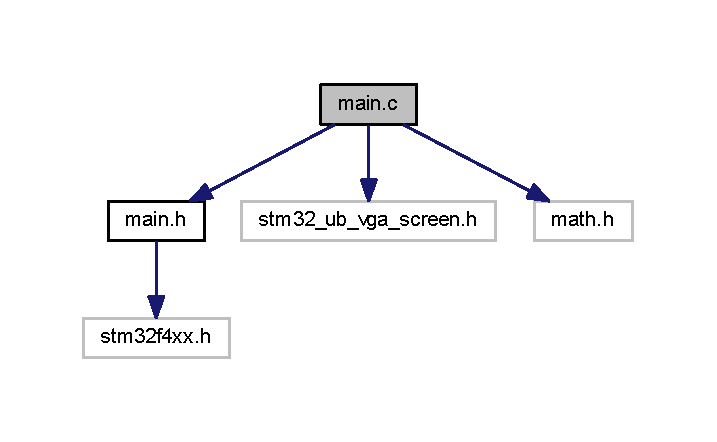
\includegraphics[width=344pt]{main_8c__incl}
\end{center}
\end{figure}
\subsection*{Functions}
\begin{DoxyCompactItemize}
\item 
int \mbox{\hyperlink{main_8c_a840291bc02cba5474a4cb46a9b9566fe}{main}} (void)
\end{DoxyCompactItemize}


\subsection{Function Documentation}
\mbox{\Hypertarget{main_8c_a840291bc02cba5474a4cb46a9b9566fe}\label{main_8c_a840291bc02cba5474a4cb46a9b9566fe}} 
\index{main.\+c@{main.\+c}!main@{main}}
\index{main@{main}!main.\+c@{main.\+c}}
\subsubsection{\texorpdfstring{main()}{main()}}
{\footnotesize\ttfamily int main (\begin{DoxyParamCaption}\item[{void}]{ }\end{DoxyParamCaption})}

\begin{DoxyDate}{Date}
24.\+04.\+2018  Niek Ratering Arntz \& Matthijs Daggelders 
\end{DoxyDate}

\begin{DoxyCode}
 */
    SystemInit(); \textcolor{comment}{// System speed to 168MHz}

    UB\_VGA\_Screen\_Init(); \textcolor{comment}{// Init VGA-Screen}

  UB\_VGA\_FillScreen(VGA\_COL\_BLACK);
  UB\_VGA\_SetPixel(10,10,10);
\end{DoxyCode}
 
%--- End generated contents ---

% Index
\backmatter
\newpage
\phantomsection
\clearemptydoublepage
\addcontentsline{toc}{chapter}{Index}
\printindex

\end{document}
